\documentclass[11pt,a4paper]{article}
\usepackage[utf8]{inputenc}
\usepackage[T1]{fontenc}
\usepackage[brazilian]{babel}
\usepackage{lmodern}
\usepackage[margin=2cm]{geometry}
\usepackage{amsmath,amssymb}
\usepackage{booktabs}
\usepackage{graphicx}
\usepackage{xcolor}
\usepackage{titlesec}
\usepackage{tabularx}
\usepackage{float}
\usepackage{tikz}
\usetikzlibrary{positioning,arrows.meta,calc,fit,backgrounds}
\usepackage{hyperref}
\usepackage{microtype}

\hypersetup{
    colorlinks=true,
    linkcolor=blue!70!black,
    citecolor=blue!70!black,
    urlcolor=blue!70!black
}

\titleformat{\section}{\large\bfseries}{\thesection.}{0.5em}{}
\titleformat{\subsection}{\normalsize\bfseries}{\thesubsection.}{0.5em}{}
\titlespacing*{\section}{0pt}{1.2ex plus 0.5ex minus .2ex}{0.6ex}
\titlespacing*{\subsection}{0pt}{1.0ex plus 0.4ex minus .2ex}{0.4ex}

\setlength{\parskip}{0.45em}
\setlength{\parindent}{0pt}

% Estilos dos diagramas
\tikzset{
    layer/.style={draw, rounded corners=2pt, minimum height=2.6em, minimum width=3.0em,
                  align=center, font=\small, fill=#1},
    layer/.default={blue!8},
    arrow/.style={-{Stealth[length=2mm]}, thick},
    lbl/.style={font=\footnotesize, align=center},
}

\newcommand{\pend}{\textcolor{red}{\textbf{?}}}

\begin{document}

\begin{center}
    {\LARGE \textbf{Projeto 3: Geração de Imagens com Autoencoders Variacionais}} \\[0.35em]
    {\large Disciplina: Introdução às Redes Neurais Artificiais} \\[0.3em]
    \textbf{Autor:} Gabriel Bonavina (RA: 168.858)\\[0.2em]
    \textbf{Repositório:} \url{https://github.com/gbonavina/projeto-3-rna}
\end{center}
\vspace{-0.5em}
\hrule
\vspace{0.8em}

\section*{Configuração Experimental}

Este trabalho treina Autoencoders Variacionais (VAE) sobre o conjunto Fashion-MNIST e analisa o espaço latente aprendido com duas dimensionalidades, $z = 2$ e $z = 8$. O Fashion-MNIST tem imagens em tons de cinza de $28 \times 28$ pixels, divididas em dez classes de roupas e acessórios: \textit{T-shirt/top}, \textit{Trouser}, \textit{Pullover}, \textit{Dress}, \textit{Coat}, \textit{Sandal}, \textit{Shirt}, \textit{Sneaker}, \textit{Bag} e \textit{Ankle boot}. Os $60\,000$ exemplos de treino originais foram separados em $50\,000$ para treino e $10\,000$ para validação por uma permutação com semente $42$. Os $10\,000$ exemplos de teste ficaram reservados para a análise final. Os pixels foram escalados para $[0, 1]$ e nenhuma outra transformação foi aplicada.

\subsection*{O Autoencoder Variacional}

Um autoencoder comum comprime a entrada em um código e tenta reconstruí-la a partir dele. O VAE troca o código fixo por uma distribuição. O \textit{encoder} recebe a imagem $\mathbf{x}$ e devolve a média $\boldsymbol{\mu}$ e o log da variância $\log \boldsymbol{\sigma}^2$ de uma gaussiana diagonal $q_\phi(\mathbf{z} \mid \mathbf{x})$. Um ponto $\mathbf{z}$ é sorteado dessa gaussiana e o \textit{decoder} $p_\theta(\mathbf{x} \mid \mathbf{z})$ tenta reconstruir a imagem. Como o sorteio não é diferenciável, usa-se o truque da reparametrização, que escreve a amostra como uma função determinística de $\boldsymbol{\mu}$ e $\boldsymbol{\sigma}$ mais um ruído externo:
\begin{equation}
    \mathbf{z} = \boldsymbol{\mu} + \boldsymbol{\sigma} \odot \boldsymbol{\varepsilon}, \qquad \boldsymbol{\varepsilon} \sim \mathcal{N}(\mathbf{0}, \mathbf{I}).
\end{equation}

O treino minimiza o negativo do limite inferior da evidência (ELBO), que soma um termo de reconstrução e um termo de regularização:
\begin{equation}
    \mathcal{L}(\mathbf{x}) = \underbrace{-\,\mathbb{E}_{q_\phi(\mathbf{z}\mid\mathbf{x})}\big[\log p_\theta(\mathbf{x} \mid \mathbf{z})\big]}_{\text{BCE somada nos 784 pixels}} + \underbrace{D_{\mathrm{KL}}\big(q_\phi(\mathbf{z} \mid \mathbf{x}) \,\|\, \mathcal{N}(\mathbf{0}, \mathbf{I})\big)}_{-\frac{1}{2}\sum_j \left(1 + \log\sigma_j^2 - \mu_j^2 - \sigma_j^2\right)}.
\end{equation}

A entropia cruzada binária (BCE) mede a fidelidade da reconstrução. A divergência KL puxa cada posterior $q_\phi(\mathbf{z}\mid\mathbf{x})$ para perto da normal padrão, o que deixa o espaço latente contínuo e sem buracos grandes. Por isso é possível gerar imagens novas sorteando $\mathbf{z} \sim \mathcal{N}(\mathbf{0}, \mathbf{I})$ e passando o vetor pelo decoder. As duas parcelas competem: reconstruir bem pede códigos espalhados e precisos, e a KL pede códigos sobrepostos e próximos da origem.

\begin{figure}[H]
\centering
\begin{tikzpicture}[node distance=0.45cm and 0.45cm]
    \node[layer=gray!15] (x) {$\mathbf{x}$\\[-1pt]\scriptsize 784};
    \node[layer, right=of x] (e1) {\scriptsize 512};
    \node[layer, right=of e1] (e2) {\scriptsize 256};
    \node[layer=orange!15, above right=0.1cm and 0.55cm of e2] (mu) {$\boldsymbol{\mu}$\\[-1pt]\scriptsize $z$};
    \node[layer=orange!15, below right=0.1cm and 0.55cm of e2] (lv) {$\log\boldsymbol{\sigma}^2$\\[-1pt]\scriptsize $z$};
    \node[layer=green!12, right=2.3cm of e2, minimum width=5.4em] (z) {$\mathbf{z} = \boldsymbol{\mu}+\boldsymbol{\sigma}\odot\boldsymbol{\varepsilon}$\\[-1pt]\scriptsize $z$};
    \node[lbl, above=0.9cm of z] (eps) {$\boldsymbol{\varepsilon} \sim \mathcal{N}(\mathbf{0},\mathbf{I})$};
    \node[layer=red!8, right=0.6cm of z] (d1) {\scriptsize 256};
    \node[layer=red!8, right=of d1] (d2) {\scriptsize 512};
    \node[layer=red!8, right=of d2] (d3) {\scriptsize 784};
    \node[layer=gray!15, right=of d3] (xh) {$\hat{\mathbf{x}}$\\[-1pt]\scriptsize $28{\times}28$};

    \draw[arrow] (x) -- (e1);
    \draw[arrow] (e1) -- (e2);
    \draw[arrow] (e2.east) -- (mu.west);
    \draw[arrow] (e2.east) -- (lv.west);
    \draw[arrow] (mu.east) -- (z.west);
    \draw[arrow] (lv.east) -- (z.west);
    \draw[arrow, dashed] (eps) -- (z);
    \draw[arrow] (z) -- (d1);
    \draw[arrow] (d1) -- (d2);
    \draw[arrow] (d2) -- (d3);
    \draw[arrow] (d3) -- (xh);

    \begin{scope}[on background layer]
        \node[draw=blue!50, dashed, rounded corners, fit=(e1)(e2)(mu)(lv), inner sep=5pt,
              label={[lbl, blue!60!black]above:encoder $q_\phi(\mathbf{z}\mid\mathbf{x})$}] (enc) {};
        \node[draw=red!50, dashed, rounded corners, fit=(d1)(d2)(d3), inner sep=5pt,
              label={[lbl, red!60!black]above:decoder $p_\theta(\mathbf{x}\mid\mathbf{z})$}] {};
    \end{scope}
    \node[lbl, below=1.55cm of z] {perda: $D_{\mathrm{KL}}\big(\mathcal{N}(\boldsymbol{\mu},\boldsymbol{\sigma}^2) \,\|\, \mathcal{N}(\mathbf{0},\mathbf{I})\big) + \mathrm{BCE}(\hat{\mathbf{x}}, \mathbf{x})$};
\end{tikzpicture}
\caption{Arquitetura do VAE usado nos experimentos. O encoder e o decoder são MLPs espelhados; cada caixa é uma camada densa com o número de unidades indicado, seguida de ReLU. A imagem é achatada para $784$ entradas, e a sigmoide na saída mantém os pixels reconstruídos em $[0, 1]$.}
\label{fig:vae}
\end{figure}

\subsection*{Treinamento}

As duas redes têm a mesma topologia e diferem só na largura das camadas $\boldsymbol{\mu}$, $\log\boldsymbol{\sigma}^2$ e da primeira camada do decoder, o que resulta em $1\,068\,820$ parâmetros para $z = 2$ e $1\,073\,440$ para $z = 8$. O otimizador foi o Adam com taxa de aprendizado $10^{-3}$, lotes de $128$ imagens e semente $0$. O treino durou no máximo $50$ épocas, com parada antecipada quando a perda de validação passava $5$ épocas sem melhorar, e os pesos da melhor época foram restaurados. O script de busca (\texttt{src/train.py}) aceita uma grade de topologias e taxas de aprendizado, mas a versão final rodou uma única configuração por dimensão latente, a descrita acima.

Toda a análise do espaço latente usa a média $\boldsymbol{\mu}$ do encoder como representação de cada imagem, para que os gráficos não dependam do ruído da amostragem. A separação entre classes foi medida de duas formas. O coeficiente de silhueta usa os rótulos verdadeiros como agrupamentos e compara a distância média de um ponto à própria classe com a distância à classe vizinha mais próxima; ele vale $1$ para classes compactas e afastadas, perto de $0$ para classes sobrepostas e fica negativo quando os pontos estão mais perto de outra classe. A acurácia de um classificador $k$-NN ($k = 10$), ajustado nos códigos da validação e avaliado nos do teste, mede se os vizinhos próximos de cada ponto são da mesma classe. Os rótulos não participam do treino do VAE em nenhum momento.

\subsection*{Métricas de fidelidade}

As perdas são dadas em nats por imagem. O nat é a unidade de informação obtida com o logaritmo natural, e $1$ nat equivale a $1/\ln 2 \approx 1{,}44$ bit. Como a BCE e a KL usam $\ln$ e somam sobre os $784$ pixels, uma $-$ELBO de $238$ nats corresponde a $238 / (784 \ln 2) \approx 0{,}44$ bit por pixel. É a grandeza que o treino otimiza, mas ela não diz diretamente o quanto as imagens se parecem. Por isso foram usadas também três métricas de imagem:
\begin{enumerate}
    \item \textbf{PSNR} (\textit{Peak Signal-to-Noise Ratio}): $10 \log_{10}(1/\mathrm{MSE})$ entre cada imagem de teste e sua reconstrução a partir de $\boldsymbol{\mu}$, com pixels em $[0, 1]$, em média sobre o teste. Maior é melhor.
    \item \textbf{SSIM} (\textit{Structural Similarity}): compara média, variância e covariância locais (janelas gaussianas de $11 \times 11$) entre a imagem e a reconstrução. Vale $1$ para imagens idênticas e é mais sensível ao borrado e à perda de estrutura do que o PSNR.
    \item \textbf{FID} (\textit{Fréchet Inception Distance}): avalia a geração, não a reconstrução. As $10\,000$ imagens de teste e $10\,000$ amostras geradas a partir de $\mathbf{z} \sim \mathcal{N}(\mathbf{0}, \mathbf{I})$ passam pela Inception-v3, e as features de $2048$ dimensões de cada conjunto são modeladas como gaussianas. O FID é a distância de Fréchet entre elas, $\|\boldsymbol{\mu}_r - \boldsymbol{\mu}_g\|^2 + \mathrm{Tr}\big(\Sigma_r + \Sigma_g - 2(\Sigma_r\Sigma_g)^{1/2}\big)$. Menor é melhor. A Inception foi treinada no ImageNet, então as imagens são ampliadas para $299 \times 299$ e o canal cinza é replicado em três. Isso torna o valor comparável apenas entre os modelos deste trabalho. Como referência do melhor valor alcançável, calculou-se também o FID entre $10\,000$ imagens reais de treino e o teste.
\end{enumerate}

\section{Resultados de Treinamento}

A Tabela~\ref{tab:loss} resume as perdas e a Figura~\ref{fig:loss} mostra as curvas. O modelo com $z = 2$ parou na época $39$, com a melhor validação na época $34$. O modelo com $z = 8$ parou na época $43$, com a melhor validação na época $38$. As curvas de treino e validação ficam próximas nos dois casos, e a perda de teste é cerca de $1{,}4$ nat maior que a de validação, então não há sinal de sobreajuste relevante. A validação do $z = 2$ tem picos isolados nas épocas $31$ e $35$, dos quais o modelo se recupera na época seguinte. Como a avaliação também sorteia $\mathbf{z}$, parte dessa oscilação é ruído da própria medida.

\begin{table}[H]
\centering
\caption{Perda por amostra (em nats) dos melhores modelos. A $-$ELBO é a soma da BCE com a KL.}
\label{tab:loss}
\small
\begin{tabular}{lrrrrrrr}
\toprule
 & & \multicolumn{3}{c}{Validação} & \multicolumn{3}{c}{Teste} \\
\cmidrule(lr){3-5} \cmidrule(lr){6-8}
Modelo & Épocas & $-$ELBO & BCE & KL & $-$ELBO & BCE & KL \\
\midrule
VAE $z = 2$ & 39 (melhor: 34) & 253,63 & 246,94 & 6,69  & 254,95 & 248,27 & 6,68 \\
VAE $z = 8$ & 43 (melhor: 38) & 236,98 & 223,98 & 12,99 & 238,46 & 225,48 & 12,98 \\
\bottomrule
\end{tabular}
\end{table}

Passar de $2$ para $8$ dimensões reduz a BCE de teste em $22{,}8$ nats e aumenta a KL em $6{,}3$ nats, uma melhora líquida de $16{,}5$ nats na $-$ELBO. Com mais dimensões, o encoder consegue guardar mais informação sobre cada imagem e paga por isso no termo de regularização. A Figura~\ref{fig:recon} mostra o efeito. Com $z = 2$ as reconstruções guardam silhueta e brilho médio, mas perdem detalhes e às vezes trocam o tipo de calçado: a sandália da terceira coluna volta como um tênis. Com $z = 8$ a sandália mantém as tiras, a bota ganha contorno e sola, e a camisa clara da penúltima coluna ganha recortes e gola que somem com $z = 2$. Estampas e texturas finas se perdem nos dois modelos, o que é esperado de um decoder que trata cada pixel como uma Bernoulli independente: ele aprende a média dos casos possíveis, e a média sai borrada.

A Tabela~\ref{tab:fid} traz as métricas de imagem. O PSNR sobe de $16{,}80$ para $19{,}57\,\mathrm{dB}$ e o SSIM de $0{,}642$ para $0{,}768$, o que confirma em números o que a Figura~\ref{fig:recon} mostra.

\begin{table}[H]
\centering
\caption{Fidelidade das reconstruções (PSNR e SSIM, conjunto de teste) e qualidade das amostras geradas (FID contra o teste). FID entre imagens reais de treino e de teste: \pend.}
\label{tab:fid}
\small
\begin{tabular}{lrrr}
\toprule
Modelo & PSNR (dB) & SSIM & FID \\
\midrule
VAE $z = 2$ & 16,80 & 0,642 & \pend \\
VAE $z = 8$ & 19,57 & 0,768 & \pend \\
\bottomrule
\end{tabular}
\end{table}

\begin{figure}[H]
\centering
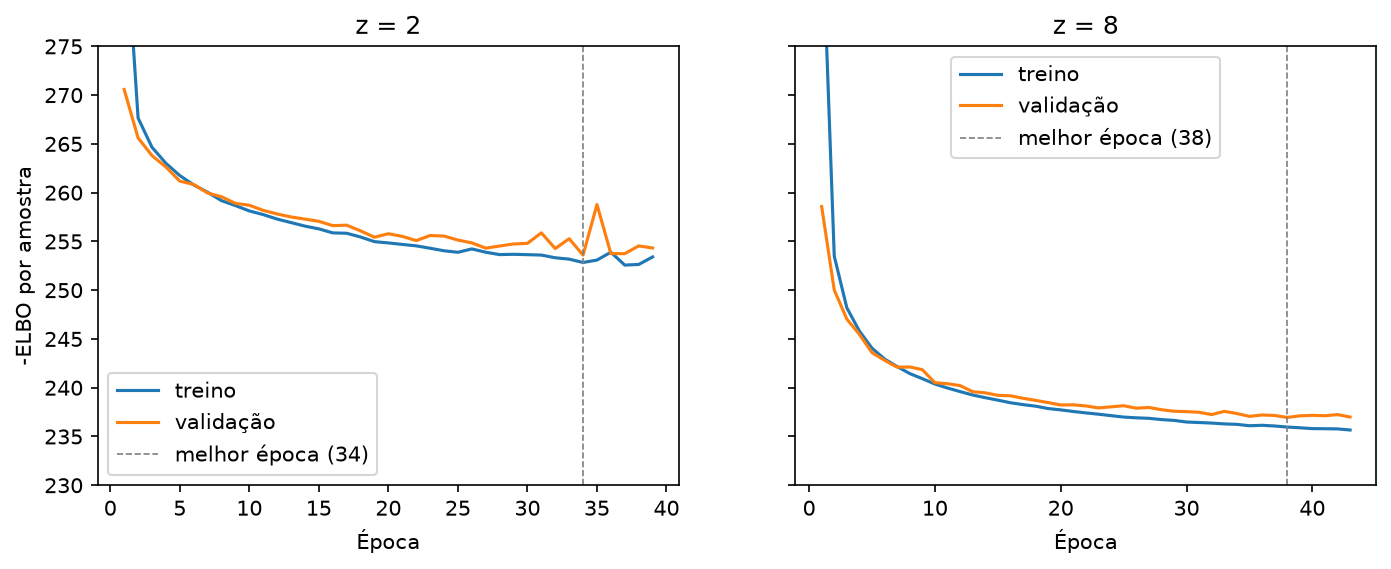
\includegraphics[width=0.95\textwidth]{../results/loss_curves.png}
\caption{$-$ELBO por amostra no treino e na validação ao longo das épocas. A linha tracejada marca a época cujos pesos foram mantidos.}
\label{fig:loss}
\end{figure}

\begin{figure}[H]
\centering
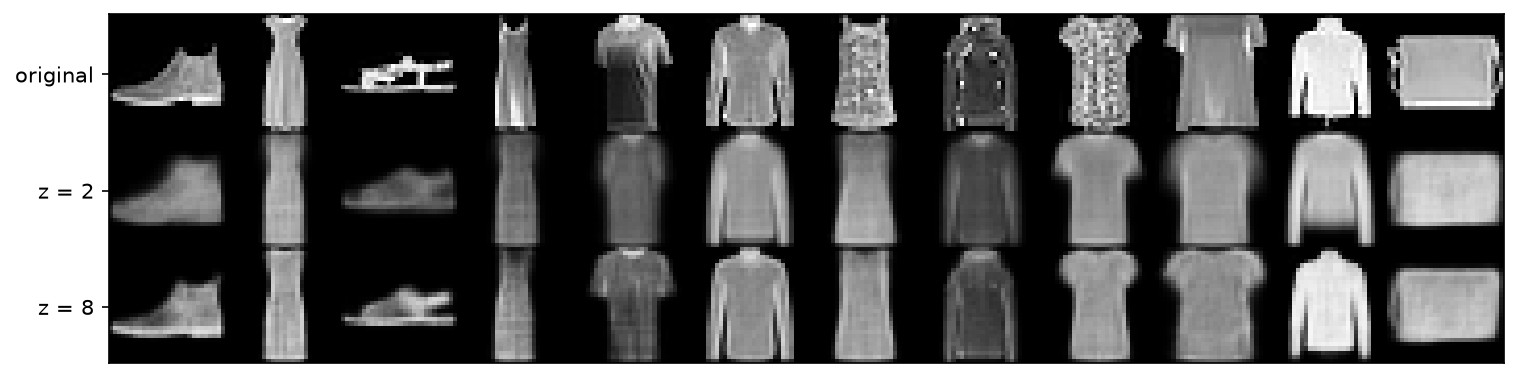
\includegraphics[width=\textwidth]{../results/reconstructions.png}
\caption{Doze imagens do conjunto de teste (primeira linha) e suas reconstruções a partir de $\boldsymbol{\mu}$ pelos VAEs com $z = 2$ e $z = 8$.}
\label{fig:recon}
\end{figure}

A Figura~\ref{fig:samples} mostra amostras geradas a partir de $\mathbf{z} \sim \mathcal{N}(\mathbf{0}, \mathbf{I})$. As do modelo $z = 2$ são todas reconhecíveis e borradas. As do modelo $z = 8$ têm mais variedade e detalhe, mas algumas saem como manchas que não lembram nenhuma classe. Em $8$ dimensões a distribuição agregada dos códigos de treino não cobre toda a massa da normal padrão, e um sorteio às vezes cai numa região que o decoder quase não viu durante o treino.

\begin{figure}[H]
\centering
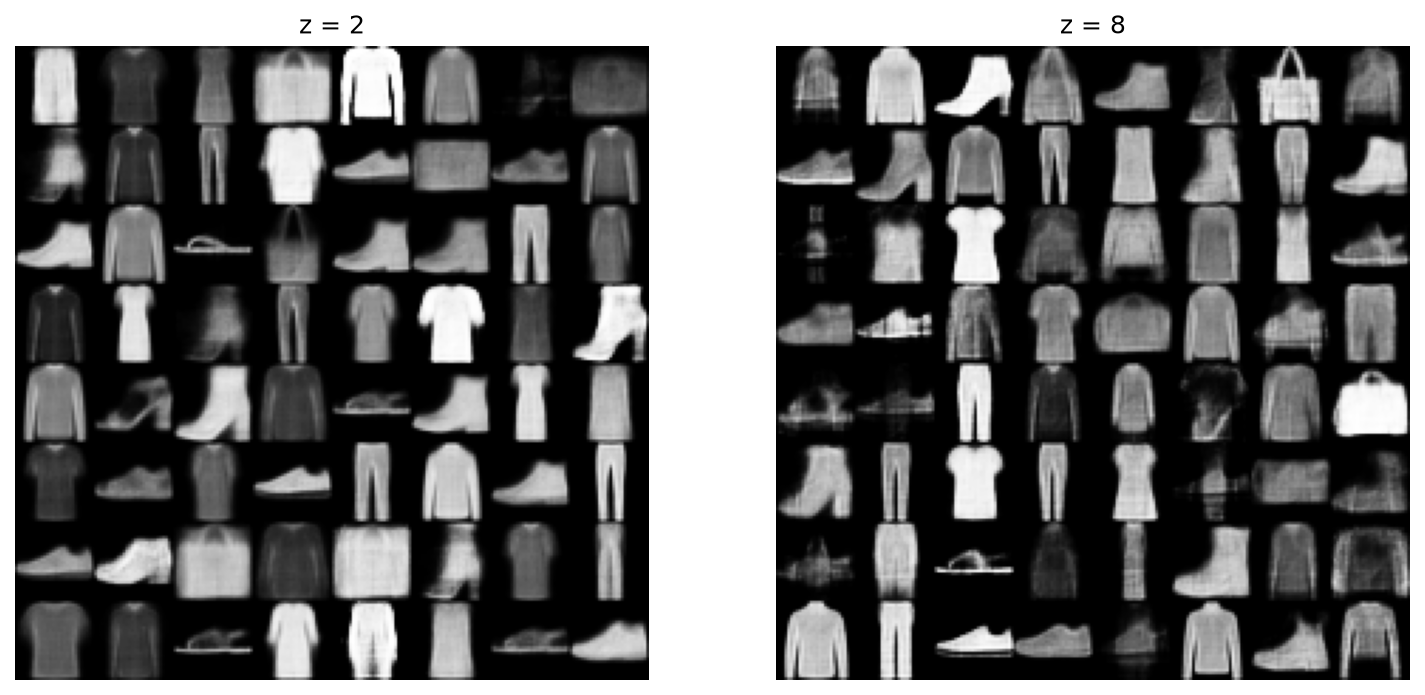
\includegraphics[width=\textwidth]{../results/samples.png}
\caption{Sessenta e quatro amostras geradas por cada modelo a partir de $\mathbf{z} \sim \mathcal{N}(\mathbf{0}, \mathbf{I})$.}
\label{fig:samples}
\end{figure}

\section{Espaço Latente com $z = 2$}

Com duas dimensões o próprio espaço latente pode ser desenhado sem nenhuma projeção (Figura~\ref{fig:latent2}). As classes se organizam em setores ao redor da origem. \textit{Trouser} forma um grupo isolado no canto superior esquerdo. Os calçados ficam à direita, com \textit{Sneaker} acima, \textit{Sandal} à esquerda e \textit{Ankle boot} à direita, e \textit{Bag} ocupa a região inferior direita. As peças de cima (\textit{T-shirt/top}, \textit{Pullover}, \textit{Coat}, \textit{Shirt} e \textit{Dress}) dividem o lado esquerdo e inferior e se sobrepõem bastante, em especial \textit{Pullover}, \textit{Coat} e \textit{Shirt}, que têm a mesma silhueta de manga longa e diferem por detalhes que duas dimensões não comportam. O coeficiente de silhueta é $0{,}125$ e o $k$-NN acerta $72{,}9\%$ das classes no teste.

\begin{figure}[H]
\centering
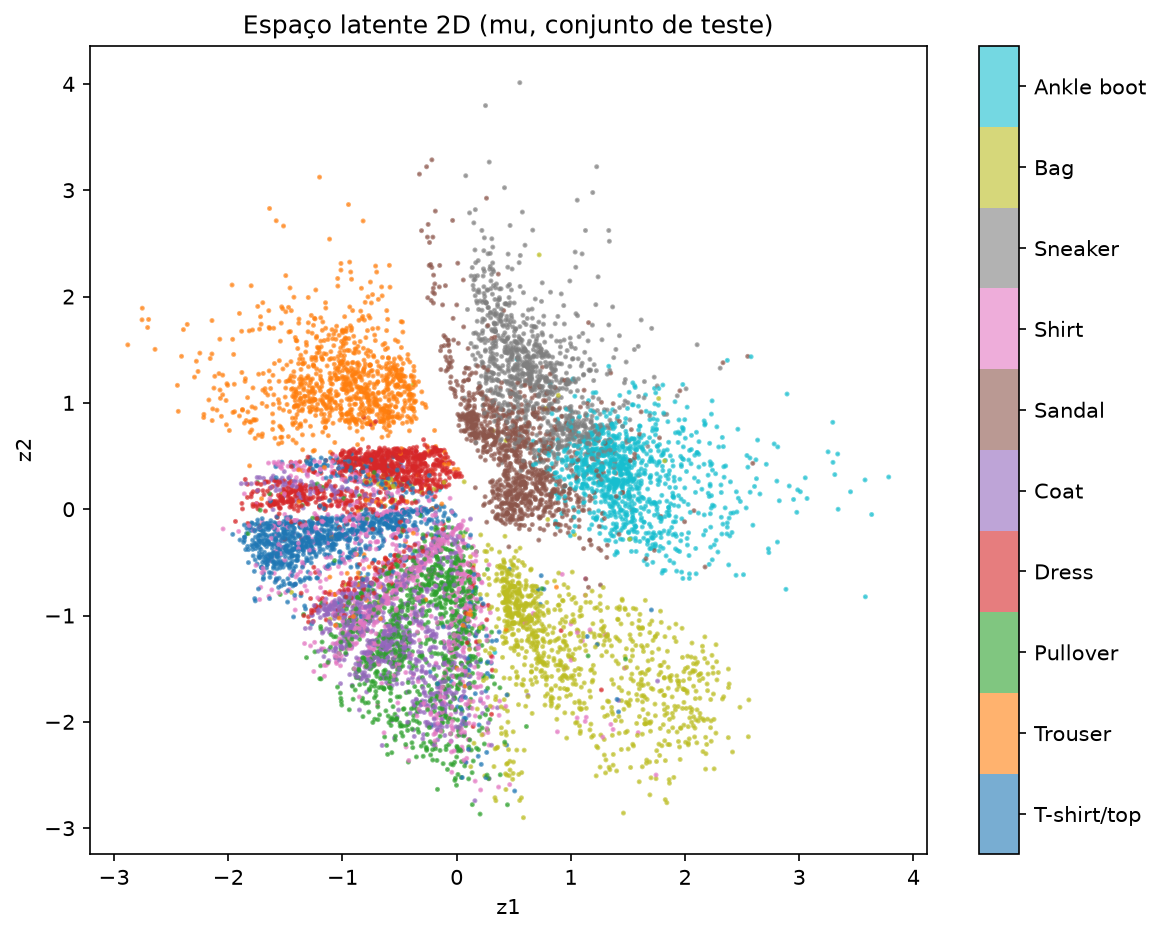
\includegraphics[width=0.78\textwidth]{../results/latent_z2.png}
\caption{Médias $\boldsymbol{\mu}$ das $10\,000$ imagens de teste no espaço latente do VAE com $z = 2$, coloridas pela classe verdadeira.}
\label{fig:latent2}
\end{figure}

O \textit{manifold} da Figura~\ref{fig:manifold} decodifica uma grade de $20 \times 20$ pontos espaçados pelos quantis de $5\%$ a $95\%$ da normal padrão em cada eixo, então cada célula ocupa a mesma massa de probabilidade do prior. A organização confere com o gráfico de dispersão: calças no alto à esquerda, tênis no alto à direita, botas e saltos no meio da direita, bolsas embaixo à direita e camisetas, vestidos e blusas à esquerda. As transições são contínuas. Descendo pela coluna da esquerda, a calça vira um vestido, depois camiseta e por fim blusa de manga longa. Na direita, o tênis ganha cano até virar bota. A ausência de regiões vazias ou imagens degeneradas na grade é efeito direto do termo KL, que mantém os códigos próximos da origem e sobrepostos.

\begin{figure}[H]
\centering
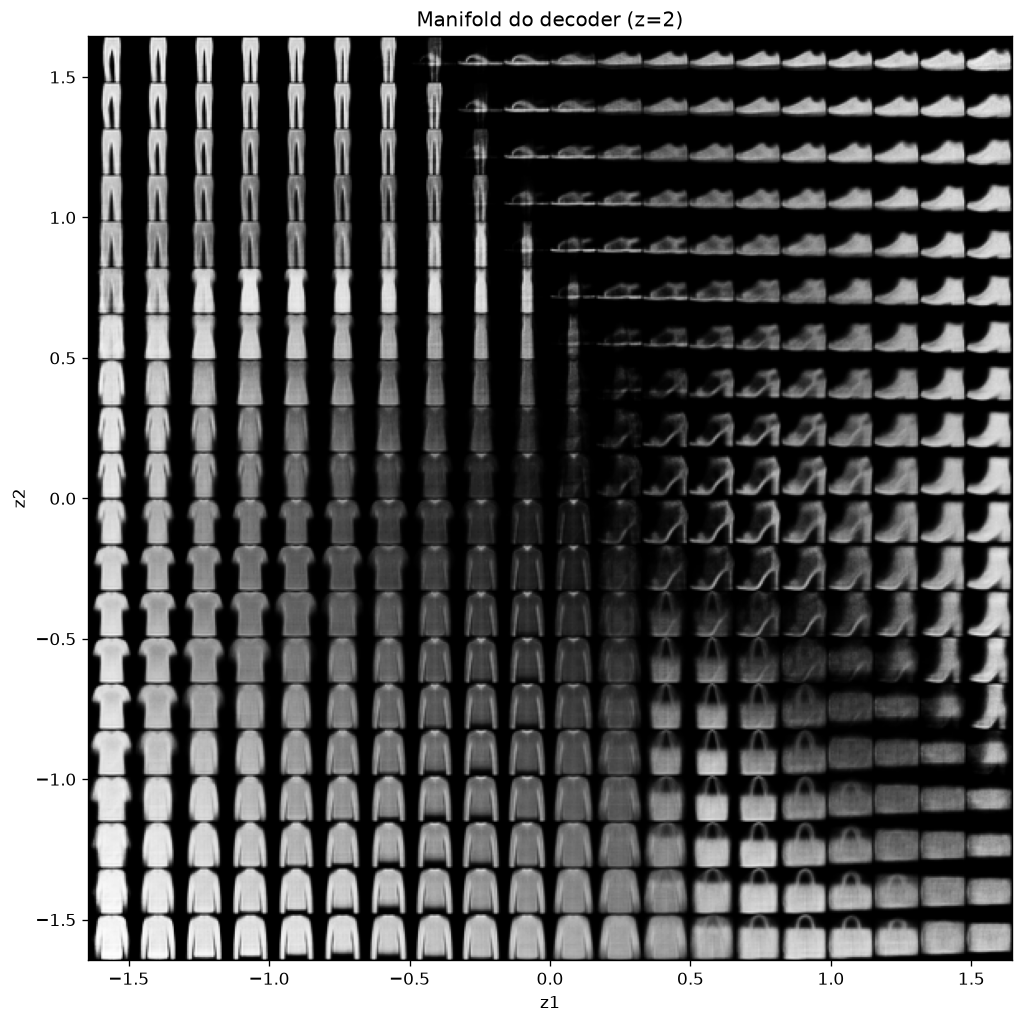
\includegraphics[width=0.72\textwidth]{../results/manifold_z2.png}
\caption{Imagens geradas pelo decoder do VAE com $z = 2$ numa grade regular nos quantis da normal padrão.}
\label{fig:manifold}
\end{figure}

\subsection{PCA com $z = 2$}

Aplicar PCA a um latente que já tem duas dimensões não reduz nada; o resultado é só uma rotação dos eixos. Ainda assim a decomposição é informativa. Ajustada sobre os códigos da validação, ela atribui $52{,}3\%$ da variância ao primeiro componente e $47{,}7\%$ ao segundo, e o desvio padrão de $\mu$ em cada eixo é $0{,}99$ e $1{,}04$. A nuvem de pontos é praticamente isotrópica, com a forma da normal padrão que a KL impõe. A informação sobre as classes está na direção angular em torno da origem (os setores da Figura~\ref{fig:latent2}), e nenhum eixo de maior variância a resume. Essa mesma propriedade é o que torna a PCA pouco útil no caso de $z = 8$.

\section{Espaço Latente com $z = 8$}

\subsection{PCA com $z = 8$}

Para visualizar um espaço de oito dimensões é preciso projetá-lo em duas. A primeira tentativa foi a PCA, ajustada nos códigos da validação e aplicada aos do teste. A Figura~\ref{fig:pcavar} mostra a variância explicada por componente: $16{,}6\%$, $15{,}8\%$, $15{,}7\%$, $14{,}9\%$, $13{,}1\%$, $13{,}0\%$, $10{,}9\%$ e $0{,}005\%$. Os dois primeiros componentes somam só $32{,}4\%$ da variância.

\begin{figure}[H]
\centering
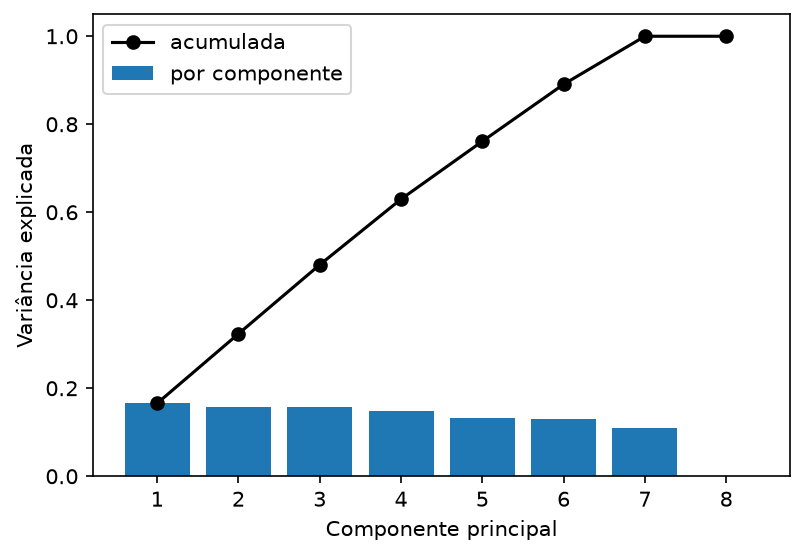
\includegraphics[width=0.55\textwidth]{../results/pca_z8_variance.png}
\caption{Variância explicada por componente principal (barras) e acumulada (linha) no latente de $8$ dimensões.}
\label{fig:pcavar}
\end{figure}

O espectro plano tem a mesma causa vista no caso de $z = 2$. A KL empurra a distribuição dos códigos para $\mathcal{N}(\mathbf{0}, \mathbf{I})$, que tem a mesma variância em todas as direções, e a PCA só sabe ordenar direções por variância. Sem direções dominantes, qualquer par de componentes descarta mais de dois terços da variação. Além disso, variância e separação de classes são coisas diferentes: a PCA é uma projeção linear não supervisionada e não tem como saber quais direções distinguem as classes.

O oitavo componente, com variância quase nula, corresponde a uma dimensão latente que o modelo deixou de usar. A Figura~\ref{fig:kl} mostra a KL média por dimensão no conjunto de teste. A terceira dimensão tem KL de $0{,}0004$ nat e desvio padrão de $\mu$ de $0{,}02$, contra valores entre $0{,}78$ e $2{,}72$ nats e desvios perto de $1$ nas outras sete. Para essa dimensão o encoder devolve $\mu \approx 0$ e $\sigma \approx 1$ para qualquer imagem, ou seja, o posterior colapsou no prior e ela não carrega informação. Esse colapso parcial é comum em VAEs: quando a reconstrução já é atendida pelas outras dimensões, a forma mais barata de reduzir a KL é desligar uma delas. O modelo de $8$ dimensões funciona, na prática, com $7$.

\begin{figure}[H]
\centering
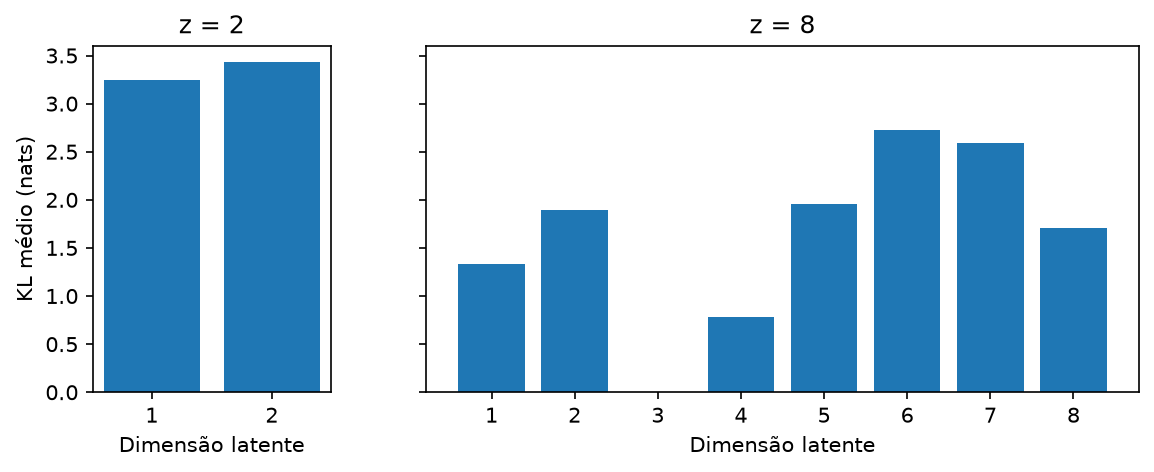
\includegraphics[width=0.75\textwidth]{../results/kl_per_dim.png}
\caption{Divergência KL média por dimensão latente no conjunto de teste. A dimensão $3$ do modelo $z = 8$ está inativa.}
\label{fig:kl}
\end{figure}

A projeção nos dois primeiros componentes (Figura~\ref{fig:pca8}) confirma o problema. Há tendências visíveis, como \textit{Trouser} e os calçados na metade superior e as peças de manga longa na inferior, mas as classes ficam sobrepostas numa nuvem única. As métricas no plano da PCA caem para silhueta de $-0{,}096$ e acurácia do $k$-NN de $33{,}9\%$. No espaço de $8$ dimensões completo, o mesmo $k$-NN acerta $81{,}8\%$. A informação de classe está lá; é a projeção linear em dois eixos que a apaga.

\begin{figure}[H]
\centering
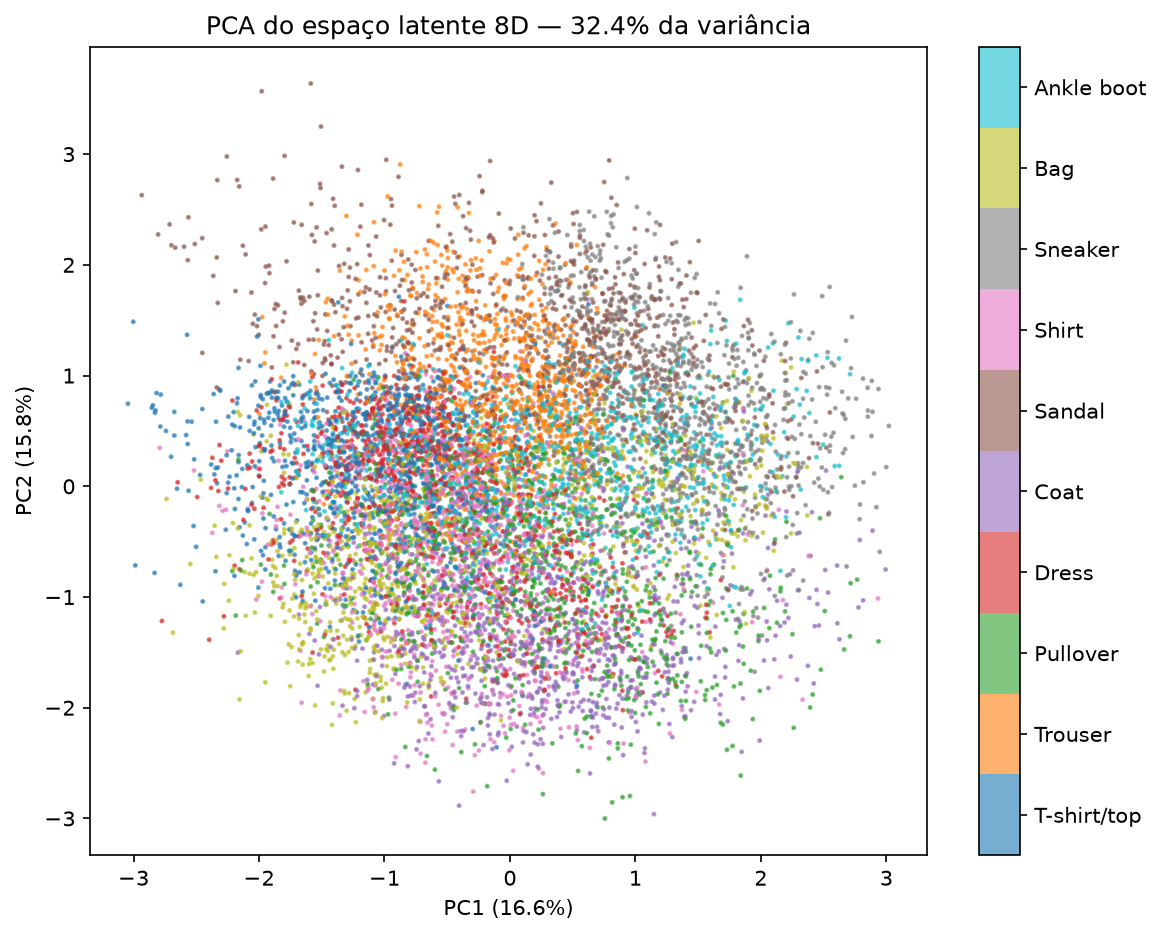
\includegraphics[width=0.78\textwidth]{../results/latent_z8_pca.png}
\caption{Projeção das médias $\boldsymbol{\mu}$ do teste nos dois primeiros componentes principais do latente de $8$ dimensões.}
\label{fig:pca8}
\end{figure}

\subsection{t-SNE com $z = 8$}

O $k$-NN mostra que, em $8$ dimensões, os vizinhos próximos de um ponto costumam ser da mesma classe. O que interessa preservar na visualização, portanto, é a vizinhança local, e é isso que o t-SNE (\textit{t-distributed Stochastic Neighbor Embedding}) faz. Ele converte as distâncias no espaço original em probabilidades de vizinhança, usando gaussianas cuja largura é ajustada para que cada ponto tenha cerca de $30$ vizinhos efetivos (a perplexidade). Depois procura uma disposição em 2D cujas probabilidades, calculadas com uma distribuição $t$ de Student, sejam as mais parecidas possíveis com as originais, minimizando a divergência KL entre as duas. A cauda pesada da distribuição $t$ permite que pontos moderadamente distantes fiquem bem afastados no plano, o que abre espaço entre os grupos. O t-SNE é não linear e não precisa que a estrutura esteja alinhada a direções de alta variância. A projeção usou os $10\,000$ códigos de teste, perplexidade $30$ e inicialização pela PCA.

\begin{figure}[H]
\centering
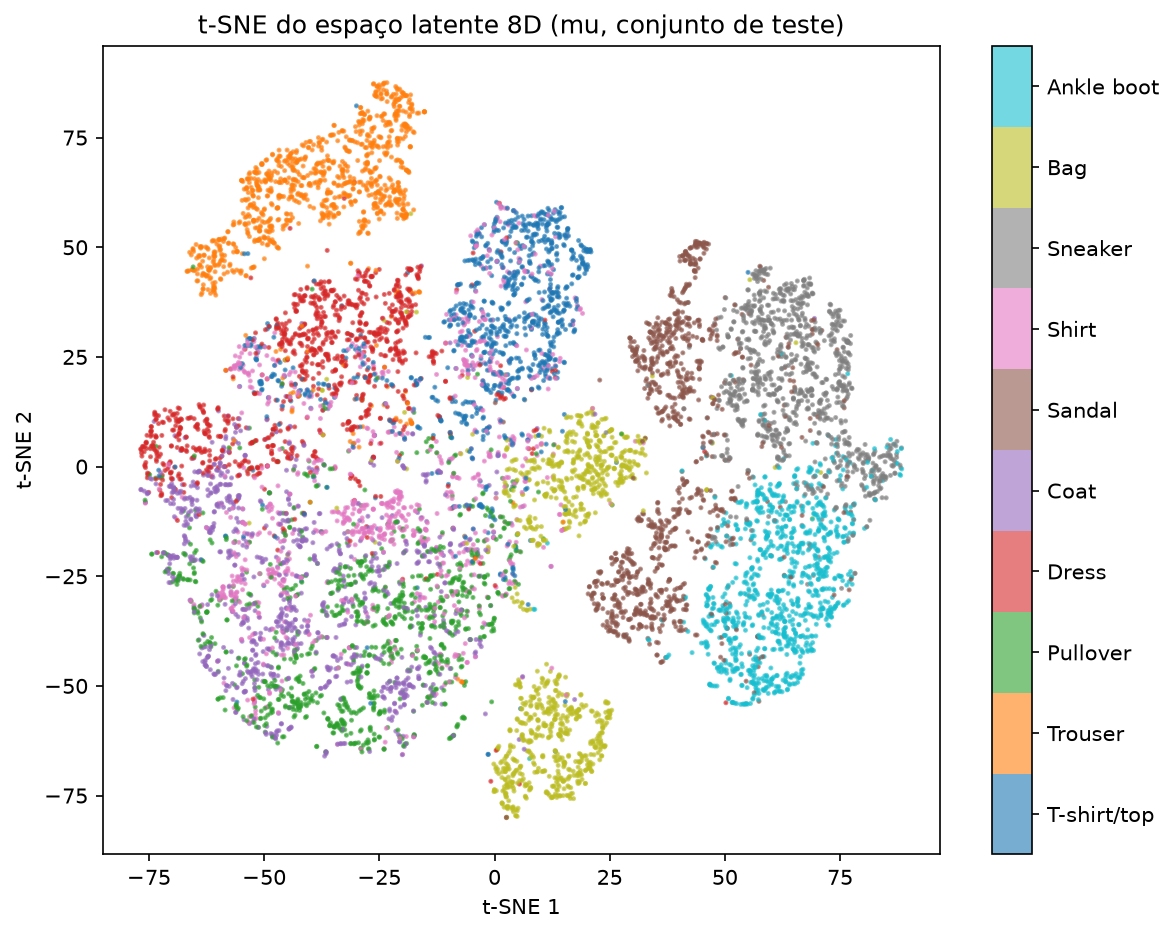
\includegraphics[width=0.78\textwidth]{../results/latent_z8_tsne.png}
\caption{Projeção t-SNE das médias $\boldsymbol{\mu}$ do teste no latente de $8$ dimensões.}
\label{fig:tsne}
\end{figure}

Na Figura~\ref{fig:tsne} os grupos aparecem com clareza. \textit{Trouser}, \textit{T-shirt/top} e \textit{Bag} formam ilhas próprias, e \textit{Bag} aparece dividida em dois grupos. À direita ficam os calçados, com \textit{Sneaker}, \textit{Ankle boot} e \textit{Sandal} em regiões distintas e vizinhas entre si; \textit{Sandal} também se divide em dois grupos. \textit{Dress} ocupa uma faixa própria entre \textit{Trouser} e as peças de cima. A sobreposição que resta está no grupo grande do canto inferior esquerdo, que mistura \textit{Pullover}, \textit{Coat} e \textit{Shirt}, e em \textit{Shirt}, cujos pontos se espalham também pelas regiões de \textit{T-shirt/top} e \textit{Dress}. É a mesma confusão vista com $z = 2$ e nas reconstruções, e corresponde a classes que diferem por detalhes pequenos.

Uma ressalva sobre a leitura do t-SNE: ele preserva quem é vizinho de quem, mas o tamanho dos grupos e a distância entre grupos diferentes no plano não têm significado quantitativo. Por isso as conclusões sobre separação se apoiam também no $k$-NN calculado no espaço original.

\subsection{Comparação entre $z = 2$ e $z = 8$}

\begin{table}[H]
\centering
\caption{Métricas de separação das classes no espaço latente (conjunto de teste). O $k$-NN foi ajustado nos códigos da validação.}
\label{tab:sep}
\small
\begin{tabular}{lrr}
\toprule
Representação & Silhueta & Acurácia $k$-NN ($k=10$) \\
\midrule
$z = 2$ (latente completo)        & 0,125    & 72,9\% \\
$z = 8$ (latente completo)        & 0,059    & 81,8\% \\
$z = 8$ (2 primeiros componentes da PCA) & $-$0,096 & 33,9\% \\
\bottomrule
\end{tabular}
\end{table}

A Tabela~\ref{tab:sep} tem um resultado que à primeira vista parece contraditório: o latente de $8$ dimensões tem silhueta menor que o de $2$, mas acurácia do $k$-NN quase $9$ pontos maior. As duas métricas medem coisas diferentes. A silhueta usa distâncias médias a todos os pontos de cada classe, e assume que as classes são aglomerados compactos e aproximadamente convexos. Em $8$ dimensões as classes ocupam regiões alongadas e de formato irregular, e as distâncias entre pontos ficam mais parecidas umas com as outras, o que achata a silhueta. O $k$-NN olha só os vizinhos imediatos e capta a estrutura local, que é melhor em $8$ dimensões. Essa é também a razão pela qual o t-SNE, que preserva vizinhanças, mostra a separação que a PCA, guiada pela variância global, não mostra.

Em resumo, o VAE com $z = 8$ reconstrói melhor, gera amostras mais detalhadas (com algumas falhas) e organiza as classes de forma mais separável localmente. O VAE com $z = 2$ reconstrói pior, mas tem um latente que pode ser inspecionado diretamente e gera amostras sempre plausíveis a partir de qualquer ponto da grade. Em nenhum dos dois as classes \textit{Pullover}, \textit{Coat} e \textit{Shirt} ficam bem separadas.

\clearpage
\appendix
\renewcommand{\thesection}{\Alph{section}}
\section{Bônus: Autoencoder Variacional Condicional (CVAE)}

O VAE gera imagens de classe aleatória, porque não há como escolher em que região do latente está a classe desejada sem antes encontrá-la. O VAE condicional (CVAE) resolve isso fornecendo o rótulo $y$ à rede. O encoder passa a modelar $q_\phi(\mathbf{z} \mid \mathbf{x}, y)$ e o decoder $p_\theta(\mathbf{x} \mid \mathbf{z}, y)$, e a função de perda é a mesma, condicionada em $y$:
\begin{equation}
    \mathcal{L}(\mathbf{x}, y) = -\,\mathbb{E}_{q_\phi(\mathbf{z}\mid\mathbf{x},y)}\big[\log p_\theta(\mathbf{x} \mid \mathbf{z}, y)\big] + D_{\mathrm{KL}}\big(q_\phi(\mathbf{z} \mid \mathbf{x}, y) \,\|\, \mathcal{N}(\mathbf{0}, \mathbf{I})\big).
\end{equation}

Na implementação (\texttt{src/cvae.py}) o rótulo entra como vetor \textit{one-hot} de $10$ posições concatenado à imagem achatada na entrada do encoder e ao vetor $\mathbf{z}$ na entrada do decoder (Figura~\ref{fig:cvae}). O resto é igual ao VAE do corpo do relatório: camadas ocultas de $512$ e $256$ unidades, Adam com taxa $10^{-3}$, lotes de $128$ e parada antecipada com paciência $5$. Foram treinadas duas versões, com $z = 2$ ($1\,076\,500$ parâmetros) e $z = 8$ ($1\,081\,120$ parâmetros), $7\,680$ a mais que o VAE correspondente por causa das entradas do rótulo.

\begin{figure}[H]
\centering
\begin{tikzpicture}[node distance=0.45cm and 0.45cm]
    \node[layer=gray!15] (x) {$\mathbf{x}$\\[-1pt]\scriptsize 784};
    \node[layer=yellow!25, below=0.5cm of x] (y) {$y$\\[-1pt]\scriptsize 10};
    \node[layer=gray!8, minimum height=6.2em, minimum width=1.1em, inner sep=1pt] (c1) at ($(x)!0.5!(y) + (1.15,0)$) {\rotatebox{90}{\scriptsize concat}};
    \node[layer, right=of c1] (e1) {\scriptsize 512};
    \node[layer, right=of e1] (e2) {\scriptsize 256};
    \node[layer=orange!15, above right=0.1cm and 0.55cm of e2] (mu) {$\boldsymbol{\mu}$\\[-1pt]\scriptsize $z$};
    \node[layer=orange!15, below right=0.1cm and 0.55cm of e2] (lv) {$\log\boldsymbol{\sigma}^2$\\[-1pt]\scriptsize $z$};
    \node[layer=green!12, right=2.5cm of e2] (z) {$\mathbf{z}$\\[-1pt]\scriptsize $z$};
    \node[lbl, above=0.9cm of z] (eps) {$\boldsymbol{\varepsilon} \sim \mathcal{N}(\mathbf{0},\mathbf{I})$};
    \node[layer=gray!8, right=of z, minimum height=6.2em, minimum width=1.1em, inner sep=1pt] (c2) {\rotatebox{90}{\scriptsize concat}};
    \node[layer=red!8, right=of c2] (d1) {\scriptsize 256};
    \node[layer=red!8, right=of d1] (d2) {\scriptsize 512};
    \node[layer=red!8, right=of d2] (d3) {\scriptsize 784};
    \node[layer=gray!15, right=of d3] (xh) {$\hat{\mathbf{x}}$\\[-1pt]\scriptsize $28{\times}28$};

    \draw[arrow] (x.east) -- (c1.west |- x.east);
    \draw[arrow] (y.east) -- (c1.west |- y.east);
    \draw[arrow] (c1) -- (e1);
    \draw[arrow] (e1) -- (e2);
    \draw[arrow] (e2.east) -- (mu.west);
    \draw[arrow] (e2.east) -- (lv.west);
    \draw[arrow] (mu.east) -- (z.west);
    \draw[arrow] (lv.east) -- (z.west);
    \draw[arrow, dashed] (eps) -- (z);
    \draw[arrow] (z) -- (c2);
    \draw[arrow, yellow!50!black] (y.south) -- ++(0,-0.9) -| (c2.south);
    \draw[arrow] (c2) -- (d1);
    \draw[arrow] (d1) -- (d2);
    \draw[arrow] (d2) -- (d3);
    \draw[arrow] (d3) -- (xh);

    \begin{scope}[on background layer]
        \node[draw=blue!50, dashed, rounded corners, fit=(e1)(e2)(mu)(lv), inner sep=5pt,
              label={[lbl, blue!60!black]above:encoder $q_\phi(\mathbf{z}\mid\mathbf{x},y)$}] {};
        \node[draw=red!50, dashed, rounded corners, fit=(d1)(d2)(d3), inner sep=5pt,
              label={[lbl, red!60!black]above:decoder $p_\theta(\mathbf{x}\mid\mathbf{z},y)$}] {};
    \end{scope}
\end{tikzpicture}
\caption{Arquitetura do CVAE. O rótulo $y$, em \textit{one-hot} com $10$ posições, é concatenado à entrada do encoder e ao código $\mathbf{z}$ antes do decoder. As ativações são as mesmas do VAE da Figura~\ref{fig:vae}.}
\label{fig:cvae}
\end{figure}

\subsection{CVAE com $z = 2$}

O treino usou as $50$ épocas disponíveis sem acionar a parada antecipada, e a melhor validação veio justamente na última época. A perda ainda caía devagar (menos de $0{,}5$ nat nas cinco últimas épocas), então um orçamento maior daria um ganho pequeno. A Tabela~\ref{tab:cvae} compara os CVAEs com os VAEs de mesma dimensão latente.

\begin{table}[H]
\centering
\caption{Comparação entre VAE e CVAE no conjunto de teste: perda por amostra (em nats), métricas de imagem e separação das classes no latente completo.}
\label{tab:cvae}
\small
\begin{tabular}{lrrrrrrrr}
\toprule
Modelo & $-$ELBO & BCE & KL & PSNR (dB) & SSIM & FID & Silhueta & $k$-NN \\
\midrule
VAE $z = 2$  & 254,95 & 248,27 & 6,68  & 16,80 & 0,642 & \pend & 0,125    & 72,9\% \\
CVAE $z = 2$ & 249,31 & 244,15 & 5,16  & 17,19 & 0,668 & \pend & $-$0,106 & 19,5\% \\
\midrule
VAE $z = 8$  & 238,46 & 225,48 & 12,98 & 19,57 & 0,768 & \pend & 0,059    & 81,8\% \\
CVAE $z = 8$ & 236,42 & 226,90 & 9,51  & 19,33 & 0,761 & \pend & $-$0,043 & 32,7\% \\
\bottomrule
\end{tabular}
\end{table}

Com $z = 2$ o CVAE reconstrói melhor (PSNR de $17{,}19$ contra $16{,}80\,\mathrm{dB}$) e usa menos KL. A classe chega ao decoder pelo rótulo, então o latente não precisa mais gastar capacidade para codificá-la. O espaço latente da Figura~\ref{fig:cvaelatent} mostra isso: as classes estão todas misturadas numa nuvem gaussiana única, e o $k$-NN acerta só $19{,}5\%$, perto dos $10\%$ de um palpite aleatório.

O $k$-NN baixo não é erro de implementação. Duas verificações confirmam que o latente perdeu a informação de classe porque ela passou para o rótulo. Decodificando os $\boldsymbol{\mu}$ do teste com os rótulos embaralhados, a BCE de reconstrução sobe de $243$ para $666$ nats, ou seja, o decoder depende do rótulo para acertar a classe. E a distância média entre os centros das classes no latente cai de $1{,}70$ no VAE para $0{,}40$ no CVAE. Comparado ao VAE da Figura~\ref{fig:latent2}, que separava as classes em setores, o latente do CVAE ficou praticamente independente do rótulo e passou a guardar a variação dentro de cada classe.

\begin{figure}[H]
\centering
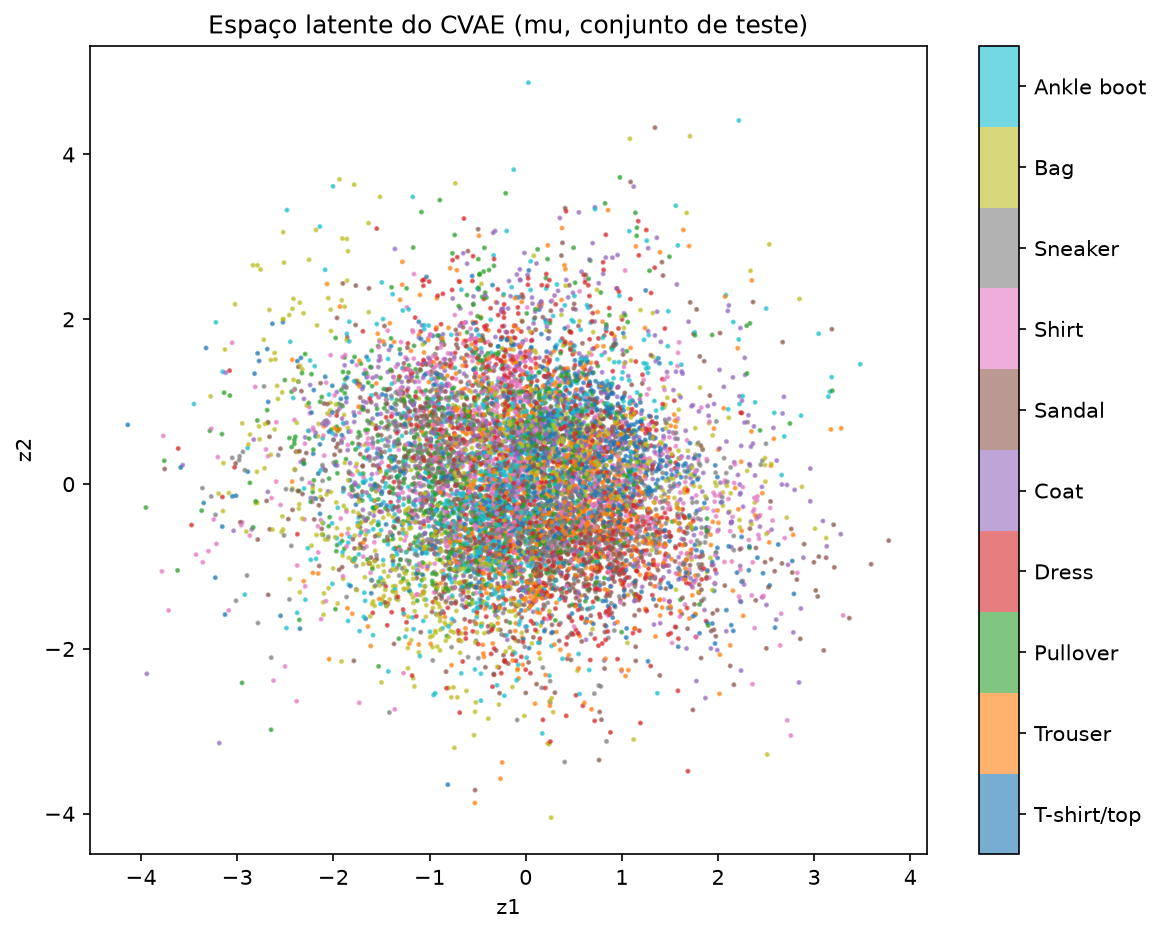
\includegraphics[width=0.7\textwidth]{../results/cvae_z2_latent.png}
\caption{Médias $\boldsymbol{\mu}$ das imagens de teste no latente do CVAE, coloridas pela classe. Ao contrário do VAE, as classes não formam grupos.}
\label{fig:cvaelatent}
\end{figure}

A Figura~\ref{fig:cvaegen} mostra a geração condicionada. Cada linha fixa uma classe e cada coluna usa o mesmo $\mathbf{z}$, que percorre $z_1$ pelos quantis de $5\%$ a $95\%$ da normal com $z_2 = 0$. Todas as imagens saem da classe pedida, o que o VAE não permite. Ao longo de $z_1$ a mudança é parecida em várias classes: camisetas, vestidos e calças ficam mais claras e mais estreitas, a camisa passa de manga longa para manga curta e a bolsa ganha uma alça visível. O efeito não é idêntico em todas. Na bota o brilho varia no sentido contrário, e na sandália $z_1$ controla a altura do salto e a quantidade de material, indo de um modelo fechado e alto até uma sandália rasteira quase vazia. O decoder aprendeu a interpretar o mesmo código de forma diferente conforme o rótulo.

\begin{figure}[H]
\centering
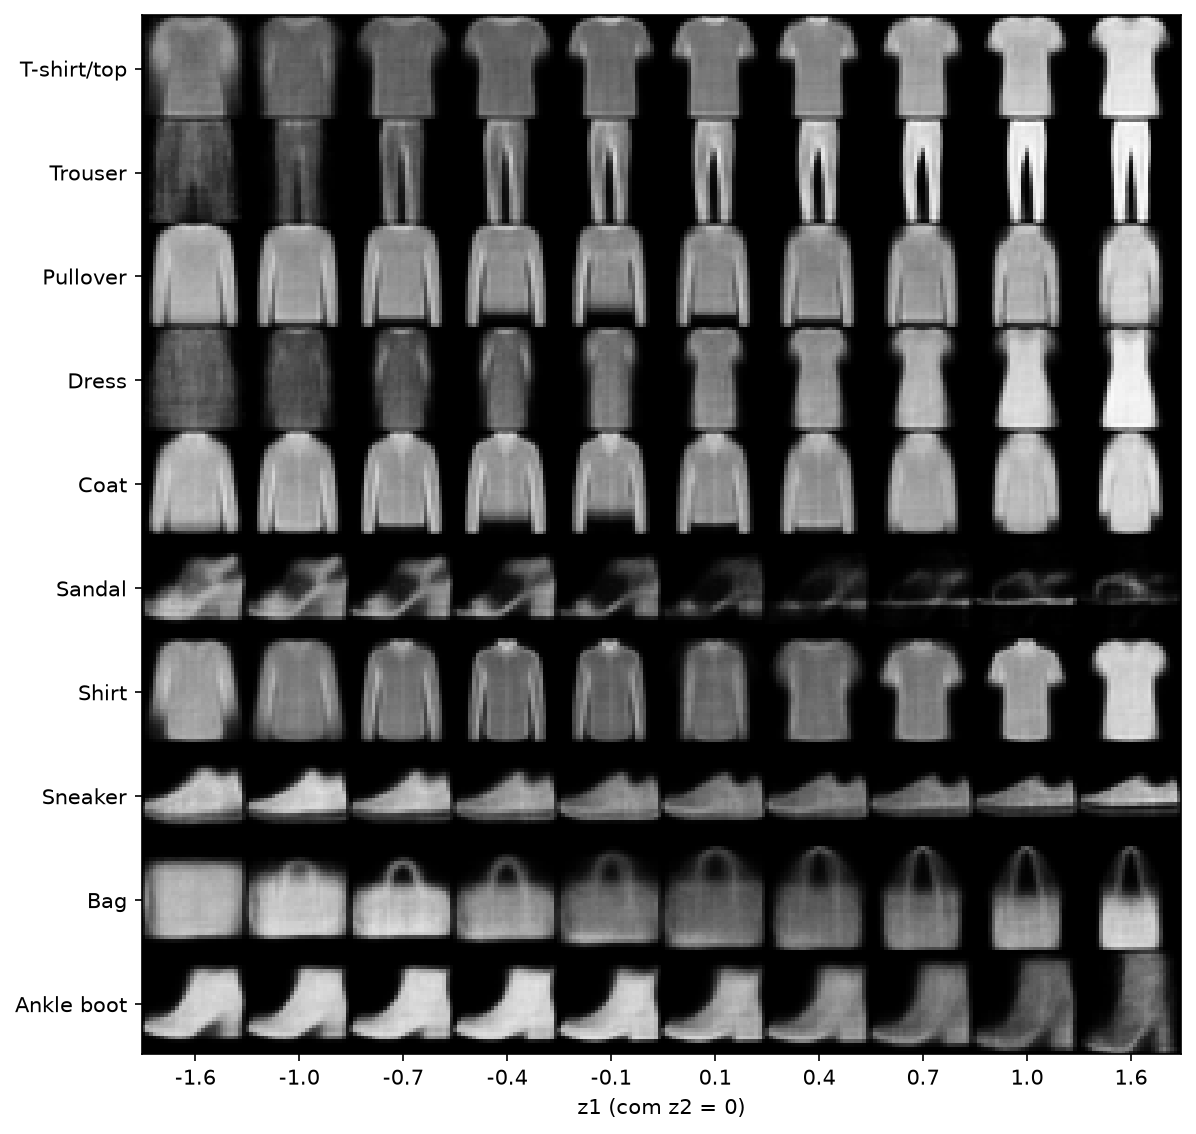
\includegraphics[width=0.78\textwidth]{../results/cvae_z2_generation.png}
\caption{Imagens geradas pelo CVAE com $z = 2$. Cada linha condiciona em uma classe e cada coluna usa o mesmo ponto $\mathbf{z} = (z_1, 0)$.}
\label{fig:cvaegen}
\end{figure}

\subsection{CVAE com $z = 8$: tentativa de organizar o latente para a PCA}

Na Seção~3 a PCA do VAE com $z = 8$ não mostrou as classes, e o t-SNE foi necessário para enxergar a separação. A ideia testada aqui foi treinar o CVAE com $z = 8$ para ver se a informação do rótulo deixaria o latente mais organizado e a PCA mais legível. O treino também usou as $50$ épocas, com a melhor validação na época $49$.

O resultado foi o oposto (Figura~\ref{fig:cvae8pca}). A projeção nos dois primeiros componentes, que somam $38{,}8\%$ da variância, é uma nuvem única com todas as classes misturadas. No plano da PCA o $k$-NN acerta $13{,}6\%$, contra $33{,}9\%$ do VAE, e no latente completo acerta $32{,}7\%$, contra $81{,}8\%$. É o mesmo efeito visto com $z = 2$. O CVAE recebe a classe pelo rótulo, então o treino não tem motivo para codificá-la em $\mathbf{z}$, e a KL pune qualquer informação redundante guardada ali. Condicionar o modelo tira a classe do latente em vez de organizá-lo por classe, e não sobra estrutura de classe para a PCA (nem o t-SNE) mostrar. O espectro da PCA também revela que duas dimensões colapsaram: os componentes $7$ e $8$ têm variância de $0{,}01\%$ e $0{,}007\%$, e o modelo usa só $6$ das $8$ dimensões, uma a menos que o VAE. Com a classe vindo de fora, sobra menos informação para guardar.

\begin{figure}[H]
\centering
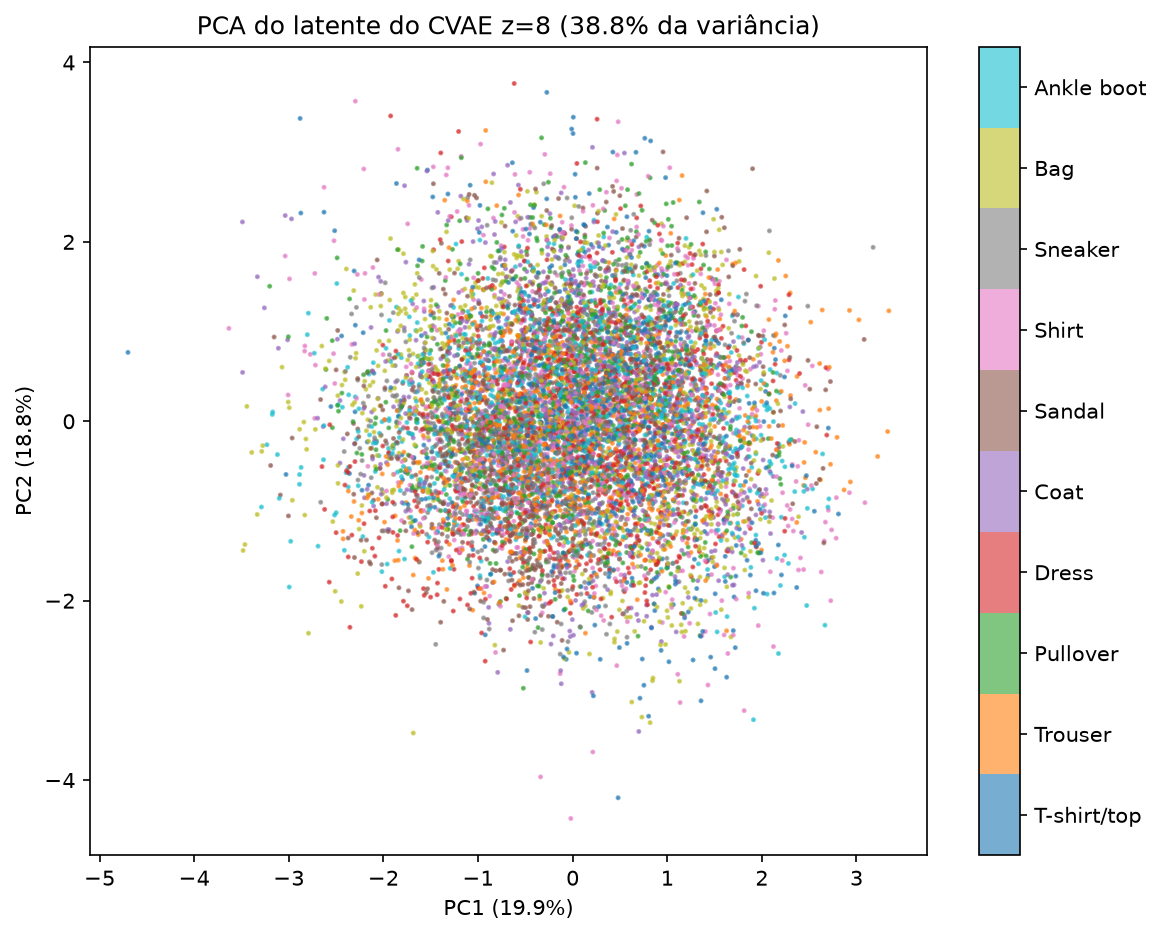
\includegraphics[width=0.7\textwidth]{../results/cvae_z8_latent.png}
\caption{Projeção PCA das médias $\boldsymbol{\mu}$ do teste no latente do CVAE com $z = 8$ (mesmo protocolo da Figura~\ref{fig:pca8}).}
\label{fig:cvae8pca}
\end{figure}

O que o latente do CVAE guarda é o estilo, e a Figura~\ref{fig:cvae8gen} deixa isso visível. Cada coluna usa um mesmo $\mathbf{z}$ sorteado da normal padrão para as dez classes, e o estilo se mantém ao longo da coluna. A quarta coluna gera, em todas as classes, peças escuras e estreitas: camiseta e blusa escuras, calça e vestido finos, sandália rasteira e bolsa pequena. A terceira gera peças largas e claras, com sandália de salto alto, bolsa quadrada grande e bota robusta. Na reconstrução, o CVAE com $z = 8$ fica praticamente empatado com o VAE (PSNR de $19{,}33$ contra $19{,}57\,\mathrm{dB}$). A $-$ELBO dele é um pouco melhor porque usa menos KL, mas a BCE é ligeiramente pior.

\begin{figure}[H]
\centering
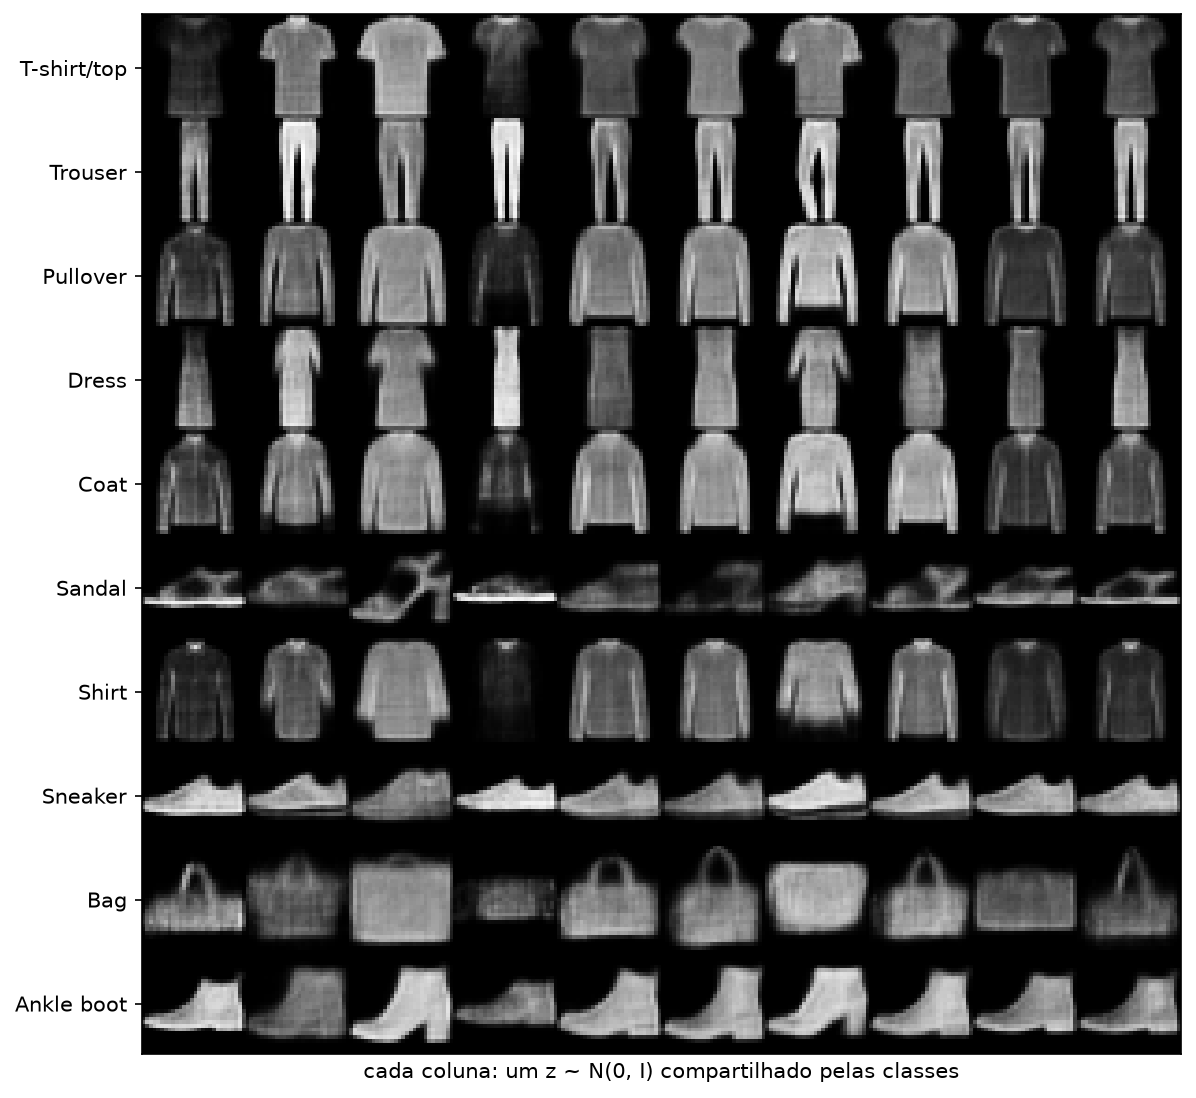
\includegraphics[width=0.78\textwidth]{../results/cvae_z8_generation.png}
\caption{Imagens geradas pelo CVAE com $z = 8$. Cada linha condiciona em uma classe e cada coluna usa o mesmo $\mathbf{z} \sim \mathcal{N}(\mathbf{0}, \mathbf{I})$.}
\label{fig:cvae8gen}
\end{figure}

Para que a PCA mostrasse as classes, o rótulo teria que agir sobre o próprio latente, e não só sobre o decoder. Um caminho é trocar o prior $\mathcal{N}(\mathbf{0}, \mathbf{I})$ por um prior por classe, $p(\mathbf{z} \mid y) = \mathcal{N}(\boldsymbol{\mu}_y, \mathbf{I})$, com médias $\boldsymbol{\mu}_y$ aprendidas. Assim a KL puxaria cada classe para um centro diferente. Outro é acrescentar à perda um classificador sobre $\mathbf{z}$. Nos dois casos a separação passa a ser imposta pelo treino, o que muda o que o latente representa, e esses modelos não foram testados neste trabalho.

\end{document}
